\chapter{Introduction} \label{chap_introduction}

Shortly after starting my bachelor's degree in 2008, I started to work as a junior
software engineer. I was confident I was willing to accept any technical challenge as my
experience up until that point led me to believe that creating some software was not that
difficult. I could not have been more wrong. I quickly discovered it was a real challenge
to apply new requirements to existing pieces of (legacy) software or explain my craftings
to the more mature engineers. The craftsmanship of software engineering was enormously
challenging to me.

Determined to overcome the difficulties, I started reading and investigating and
immediately recognized the Law of Increasing Complexity of
\textcite{lehman_programs_1980}, where he explained the balance between the forces driving
new requirements and those that slow down progress. Other pioneers in software have
recognized these challenges in engineering also.


\textcite{d_mcilroy_nato_1968} proposed a vision for systematically reusing software building
blocks that should lead to more reuse. \textcite{d_mcilroy_nato_1968} stated, \enquote{The real
hero of programming is the one who writes negative code,} i.e., when a change in a program
source makes the number of lines of code decrease ('negative' code), while its overall
quality, readability or speed improves \parencite{wikipedia_douglas_2023}. Perhaps very
early concepts of modular software constructs?

\textcite{dijkstra_letters_1968} argued against using unstructured control flow in
programming and advocated for using structured programming constructs to improve the
clarity and maintainability of the source code. In addition,
\Citeauthor{dijkstra_letters_1968} advocated structured programming techniques that
improved the modularity and evolvability of software artifacts.

\textcite{parnas_criteria_1972} continued with the principle of information hiding.
\Citeauthor{parnas_criteria_1972} stated that design decisions used multiple times by a
software artifact should be modularized to reduce complexity. 

Over the years, I got introduced to various software design principles and philosophies
like \gls{ca}, increasing my knowledge and craftsmanship. My career moved more toward
architecture and product management. Nevertheless, I have always retained my passion for
Software Engineering.

My obsession got re-ignited during the Master's degree introduction days at the Priory of
Corsendock. Jan Verelst introduced me to \gls{ns}, and I was intrigued by software
stability and evolvability. It was fascinating to learn that there is now empirical
scientific evidence for a quest I have been on for almost a decade. 

\gls{ns} Had to be the topic of my research. I was curious to compare what I knew
(\gls{ca}) with what science offered (\gls{ns}). In early investigations, I found
overlapping characteristics. Nevertheless, there were also a couple of differences. Could
these design approaches be used in conjunction with each other?

Java SE has primarily been used for case studies in order to develop the Normalized
Systems Theory \parencite{oorts_building_2014, de_bruyn_enabling_2018}. Although
sufficient in Java, I was pleased to read that both software design approaches have
formulated modular structures independent of any programming technology
\parencite{mannaert_normalized_2009,robert_c_martin_clean_2018}. So I could use my
favorite programming language C\#, to create a software artifact that supported my
research. 

Based on early investigations, I instinctively found that many applications of \gls{ca}
are a specialization of the \gls{ns} Theorems. Consequently, I hypothesized that \gls{ca}
and \gls{ns} could be used to achieve a modular, evolvable, and stable software artifact.

\begin{figure}[H]
    \centering
    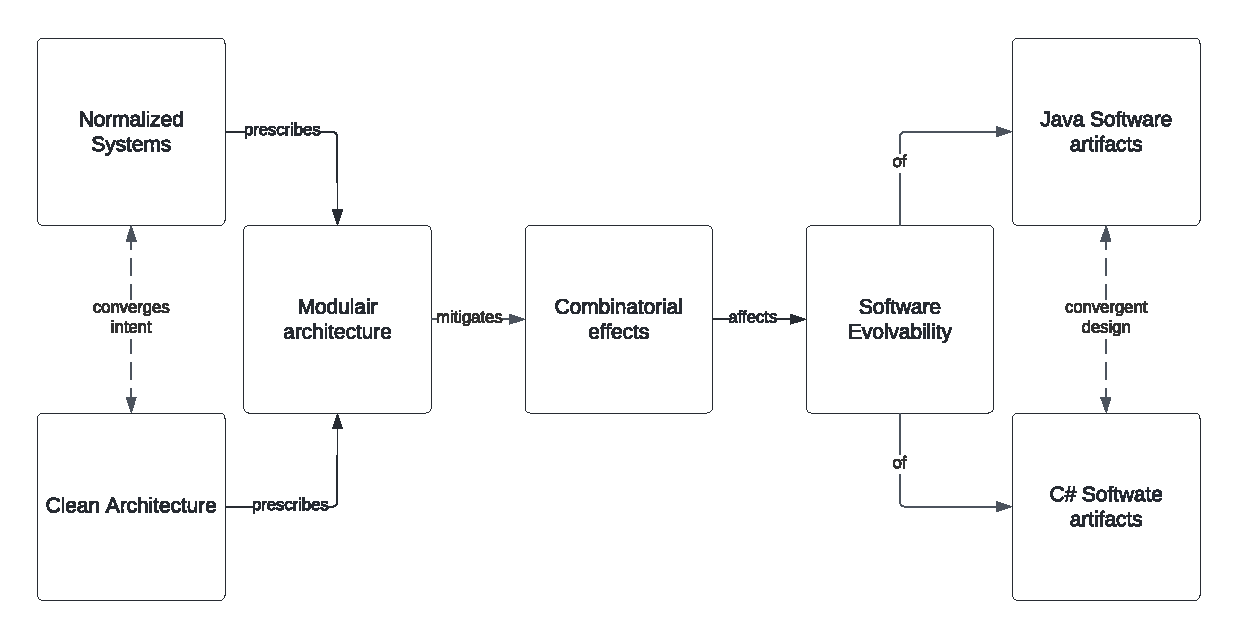
\includegraphics[width=0.8\textwidth]{figures/hypothesis.pdf}
    \caption[The hypothesis]{The hypothesis}
    \label{fig_hypothesis}
\end{figure}

Since this research is investigating the convergence of gls{ca} and \gls{ns}, it is
relevant to introduce them and discuss the concepts mentioned in the following sections.

\section{Research method} \label{sec_research_method}

This research is a Design Science Method and relies on the Engineering Cycles as described
by \textcite{wieringa_design_2014}. The engineering cycle provides a structured approach
to developing the required artifacts to analyze the design problem.

\begin{figure}[H]
    \centering
    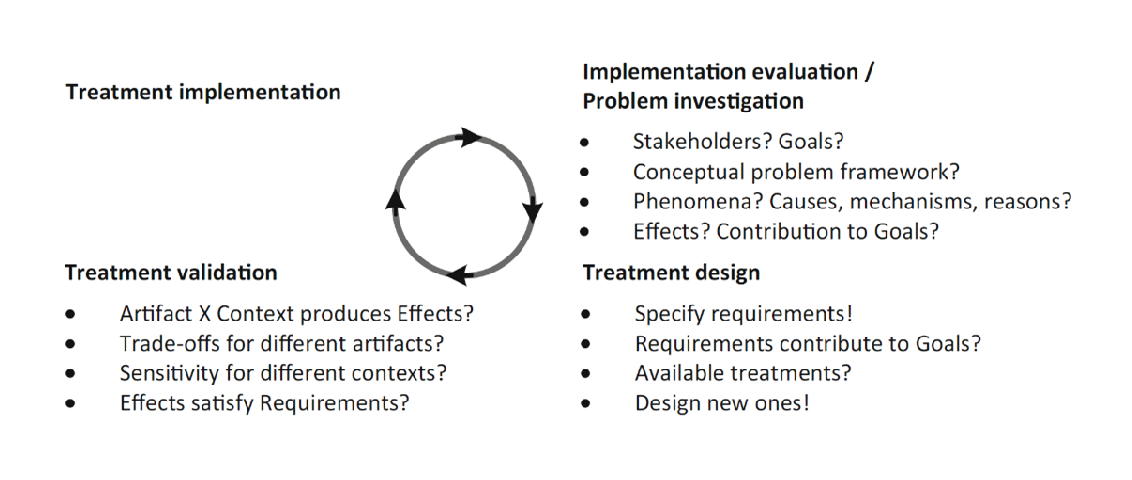
\includegraphics[width=1\textwidth]{figures/engineering_cycle.pdf}
    \caption[Engineering cycle]{The Engineering Cycle of \textcite{wieringa_design_2014}}
    \label{fig_engineering_cycle}
\end{figure}

In the course of this research, a significant component has been the development of a
tangible software artifact, providing a real-world illustration of the convergence between
Clean Architecture and Normalized Systems. \textcite{hevner_design_2004} proposed a
framework for research in information systems by introducing the interacting relevance and
rigor cycles.

Figure \ref{fig_dsr} depicts a specialization of the Design Science Framework of
\textcite{hevner_design_2004}. The rigor cycle comprises the theories and knowledge from
\gls{ns} and \gls{ca}, supplemented by the rigorous knowledge of modularity, evolvability,
and stability of software systems. The relevance cycle represents the business needs of
the stakeholders. The research requirements are described as research objectives.

\begin{figure}[H]
    \centering
    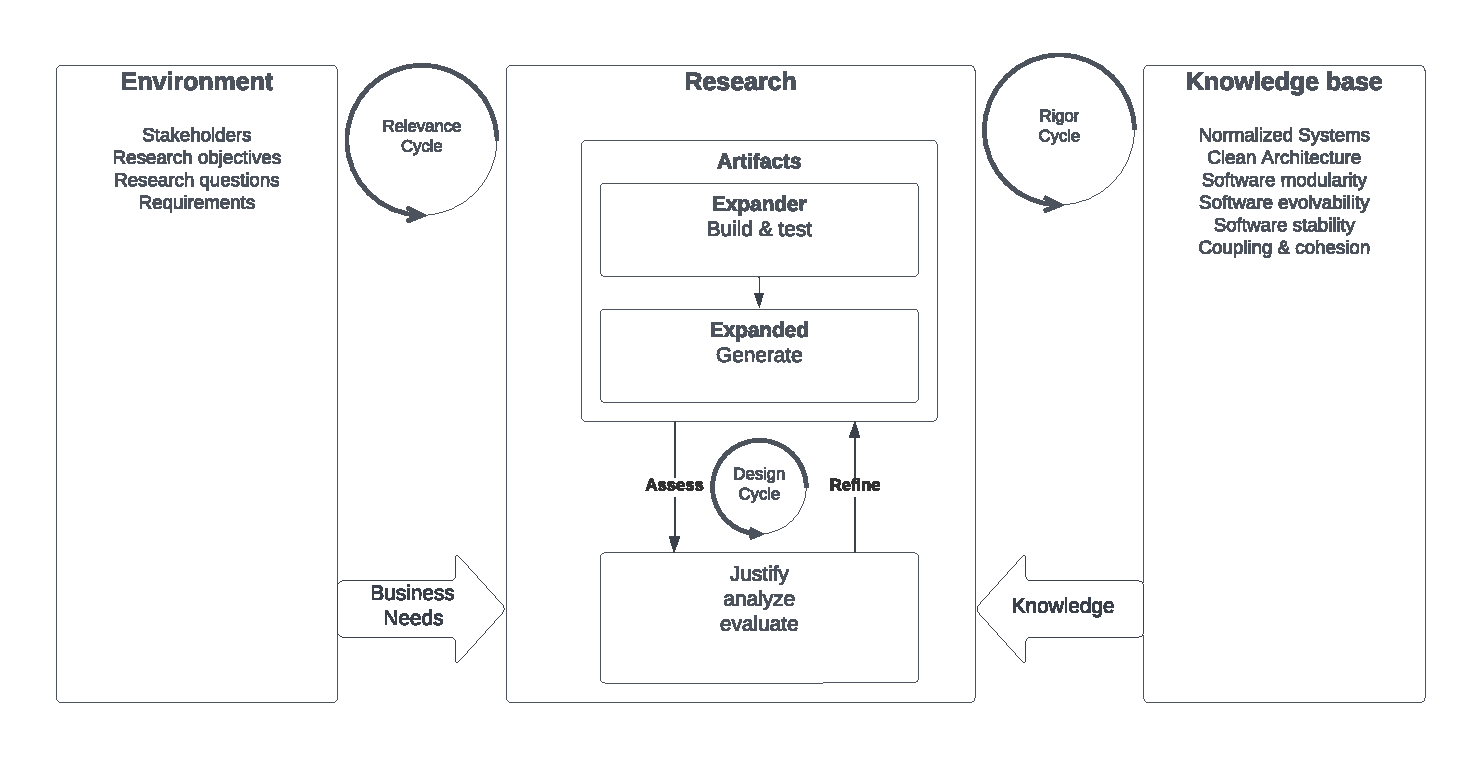
\includegraphics[width=1\textwidth]{figures/rigor_relevance_cycle.pdf}
    \caption[Design Science Framework for IS Research]{The Design Science Framework for IS Research}
    \label{fig_dsr}
\end{figure}
\section{Research Objectives} \label{sec_research_objectives}

In this Design Science Research, we will shift the focus from Research Questions to
Research Objects. The primary goal of this research is to determine the degree of
convergence of \gls{ca} with the \gls{ns} Theory. In order to achieve this goal, the
research is divided into the following objectives:

\begin{enumerate}
    \item \textbf{Literature Analysis} \newline
    Conduct a literature review of \gls{ca} and \gls{ns}, focusing on their
    fundamental elements, principles, and real-world case studies. This review will
    provide a solid foundation for understanding the underlying concepts and their
    practical implications.
    
    \item \textbf{Architectural Desing} \newline
    Create an Architectural Design fully and solely based on \gls{ca}. Implement the
    findings of the Literature Review in the Design. This design will be the basis for
    the Artifact Development.

    \item \textbf{Artifact Development} \newline
    Construct two artifacts that facilitates the study on the convergence
    between \gls{ca} and \gls{ns} Theories.
    \begin{enumerate}[label*={\arabic*.}]
        
        \item \textbf{Expander framework \& Clean Architecture Expander} \newline        
        These two components will be designed and implemented  based on the \gls{ca}
        design. The Clean Architecture Expander will enable the parameterized
        instantiation of software systems that adhere to the principles and design of
        \gls{ca}. The Expander framework serves as a supporting system for the expander,
        loading and orchestrating dependencies and models and executing the expander.
        
        \item \textbf{Expanded Clean Architecture artifact} \newline
        The expanded artifact will facilitate the analysis of a RESTful API implementation
        and its alignment with the \gls{ca} principles and design.
        
    \end{enumerate}
    
    \item \textbf{Analysis of combinatorics} \newline
    Analyze the artifacts to determine if any combinatorial effects occur due to following
    the principles and architectural approach of \gls{ca}.
\end{enumerate}
\section{Thesis outline} \label{sec_structure}

The structure of this thesis reflects the research methodology described in the previous
section \ref{sec_research_method}. Chapter \ref{chap_theoreticalbackground} presents the
theoretical backgrounds of both \gls{ns} and \gls{ca}, discussing important
characteristics and requirements of software stability, as well as the principles and
architectures proposed by both development approaches. Chapter \ref{chap_requirements}
focuses on the requirements relevant to this research. It is divided into two sections:
section \ref{sec_research_requirements} outlines the research requirements, describing the
requirements necessary for conducting the research, while section
\ref{sec_artifact_requirements} details the artifact requirements, laying out the
requirements relevant to the artifacts contributing to this research. Chapter
\ref{chap_designing_artifacts} describes all the characteristics of the design artifacts.
Chapter \ref{chap_evaluation} evaluates the research results, discussing the impact of
using CA on NS. The conclusion of this research is presented in the final chapter, Chapter
\ref{chap_conclusions}.